
\mojesekce{Open source GIS-based implementation}

\justifying
{\rmfamily The SMODERP2D model belongs to a family of so called GIS
(Geographic Information System) based hydrological models utilizing
capabilities of GIS software for geodata preprocessing. Originally the
model could run only in proprietary Esri ArcGIS platform
(\url{http://desktop.arcgis.com}). SMODERP2D project is currently
entering the open source world. The new generation of the model
presented by this contribution comes with support of two widely used
open source GIS platforms:

\begin{itemize}
\item GRASS GIS (\url{http://grass.osgeo.org}) and
\item QGIS (\url{http://qgis.org}).
\end{itemize}
}

\begin{columns}
    \begin{column}{0.5\textwidth}
    \centering
    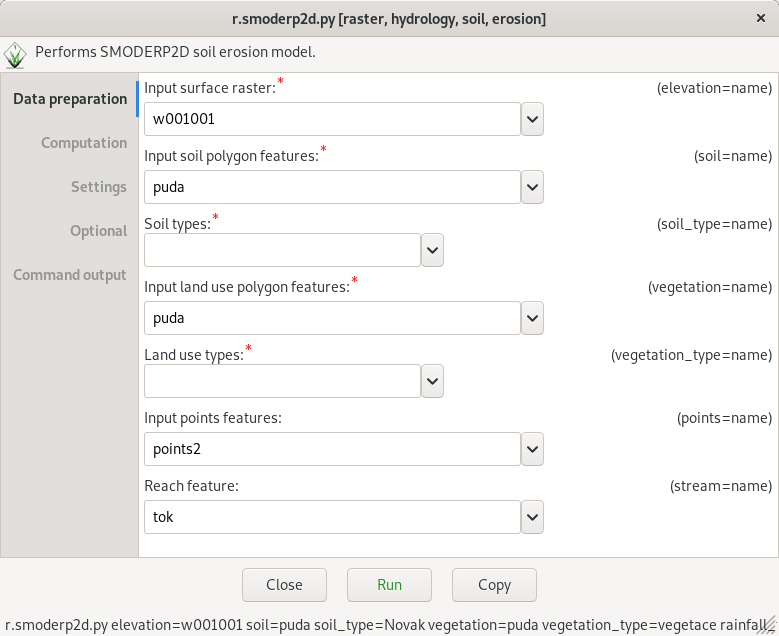
\includegraphics[width = .9\textwidth]{obr/grass.png}
    \end{column}
    \begin{column}{0.5\textwidth}
    
\includegraphics[width = .07\textwidth]{obr/grass-logo.png}
    \justifying
    {\rmfamily
    {\em GRASS} (Geographic Resources Analysis Support System) {\em
    GIS} is a free and open source GIS software suite used for
    geospatial data management and analysis, image processing, spatial
    modeling, and visualization.

    \vskip 0.5em
    
    Data preprocessing part is performed in SMODERP2D by so-called
    {\em GIS providers}. Currently there are two GIS providers
    implemented. First is based on widely used Esri proprietary
    platform, the second runs on open source GRASS GIS platform. Model
    computation including data preprocessing part can be performed in
    GRASS GIS by newly developed {\tt r.smoderp2d} GRASS Addons module.
    
    }
    \end{column}
\end{columns}

\vskip 1em

\begin{columns}
    \begin{column}{0.5\textwidth}
    
\includegraphics[width = .07\textwidth]{obr/qgis-logo.png}    
    \justifying
    {\rmfamily
    QGIS is a widely known free and open source cross-platform desktop
    geographic information system (GIS) application.

    \vskip 0.5em

    Presented QGIS plugin designed by SMODERP2D development team
    brings the model into QGIS environment while data preprocessing
    part is performed by integrated GRASS-based GIS provider.  Due to
    widely used QGIS platform, a newly developed QGIS plugin
    significantly increases accessibility of the SMODERP2D model for
    research purposes and also for engineering practice.

    }

    \end{column}
    \begin{column}{0.5\textwidth}
    \centering
    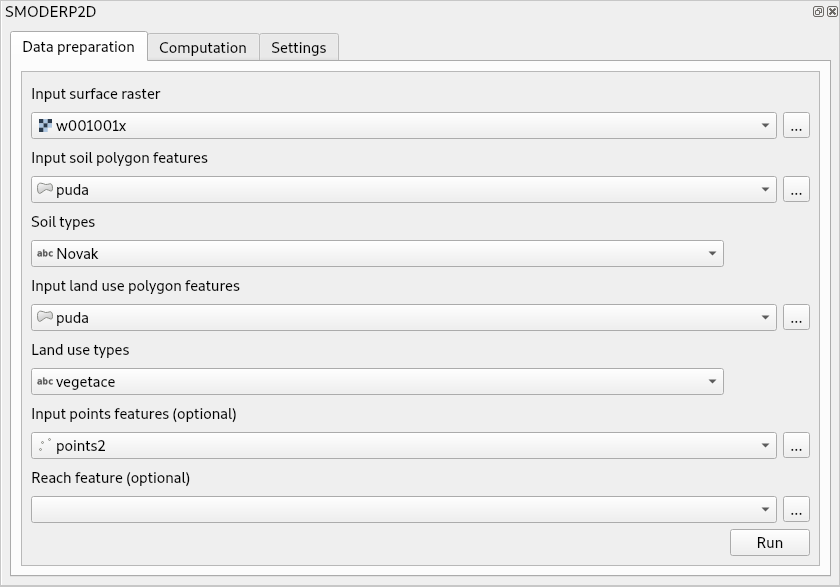
\includegraphics[width = .9\textwidth]{obr/qgis.png}
    \end{column}
\end{columns}

\mojesekce{Conclusions \& Results}

\justifying
{\rmfamily
% 
Conc
\begin{itemize}
    \item item1
    \item item2
\end{itemize}

}
      
\mojesekce{References}
\justifying
{\rmfamily
% \small{
\bibliography{lit}\vspace{0.4cm}
% }
}

\mojesekce{Acknowledgment}
\justifying
{\rmfamily
The research has been supported by the research grants SGS17/173/OHK1, TJ01000270 and QK1910029.
}



\begin{beamercolorbox}[wd=\textwidth,dp=0.25cm]{cboxb}\end{beamercolorbox}\vspace{0.5cm}


\begin{columns}
    \begin{column}{0.1\textwidth}
    \centering
    
\includegraphics[width =1\textwidth]{obr/logo_TACR_dopln_AJ.png}
    \end{column}
    \begin{column}{0.5\textwidth}
    
\includegraphics[width = 1\textwidth]{obr/LogoMZeAJ.jpg}
    \end{column}
    \begin{column}{0.4\textwidth}
    powered by
    {\tiny
    \begin{lstlisting}
       @ @ @   @       @     @ @     @ @ @     @ @ @ @  @ @ @    @ @ @
      @        @ @   @ @   @     @   @     @   @        @     @  @     @
      @        @   @   @  @       @  @      @  @        @     @  @     @
        @ @    @       @  @       @  @      @  @ @ @    @ @ @    @ @ @
            @  @       @  @       @  @      @  @        @   @    @
            @  @       @   @     @   @     @   @        @    @   @
       @ @ @   @       @     @ @     @ @ @     @ @ @ @  @     @  @

      \  \  /   / /    \   \  /   \  /    /     /        @ @ @   @ @ @
       \ _\/   /_/      \   \/     \/    /_____/        @     @  @     @
           \__/          \  /      _\___/                     @  @      @
               \____      \/      /                          @   @      @
                    \_____/______/                         @     @      @
                                 \                       @       @     @
                                  \____________________ @ @ @ @  @ @ @
    \end{lstlisting}
    }
    \end{column}
\end{columns}
